% !TeX root = ../../main.tex

\chapter{Testfälle}
\label{sec:testcases}

In diesem Abschnitt wird die entwickelte Applikation in drei Testfällen getestet.
Die Testfälle sind dabei verschiedene Szenen mit mehreren Bildern von einem Objekt, das rekonstruiert werden soll.
Die Szenen und die Objekte sind dabei so gewählt, dass sie möglichst unterschiedlich sind in Bezug auf Größe und Beschaffenheit des Objekts.
In jedem Testfall wird die Szene kurz beschrieben und die Qualität der Feature Matches, sowie ihre rekonstruierten Punkte bewertet.
Bei der Bewertung wird zu einem auf die Beschaffenheit der Szene und des Objekts und zum anderem auf die Implementierung eingegangen.
In \cref{sec:conclusion} werden die Ergebnisse der Testfälle zusammengefasst.

\section{Fall 1: Sessel}
\label{sec:textcase-chair}\ohead{Jan Maier}
Im ersten Testfall wird versucht einen Sessel zu rekonstruieren.
Dazu werden 10 Bilder verwendet, welche den Sessel aus verschiedenen Winkeln zeigt.
Die Bilder sind so sortiert, dass die Bewegung zwischen zwei Bildern minimal ist.
Die Anzahl der Matches, der rekonstruierten Punkte, sowie die Anzahl der Weltpunkte, die für die Skalierung genutzt wurden, so wie Skalierung selbst werden in \cref{tab:chair-results} gezeigt. % TODO: rewording
Das erste Bildpaar des Sessels wird in \cref{fig:chair-first-pair} gezeigt.
In \cref{fig:chair-first-pair-with-matches} wird das selbe Bildpaar mit allen Keypoints und ihren Matches gezeigt.
Matches sind dabei durch Linien gekennzeichnet, die die korrespondierenden Bildpunkte miteinander verbinden.
Hier fällt auf, dass sich die Matches überwiegend auf den Seiten des Sessels befinden.
Auch der Text auf der Decke und dem Kissen, so wie das karierte Muster des anderen Kissens werden als Keypoints erkannt und gematcht. % todo: rewording.
Des Weiteren sind viele Keypoints und Matches auf dem Teppich unten im Bild zu erkennen.
Im Gegensatz dazu gibt es sehr wenige Matches auf dem Boden, der Heizung, der Wand, sowie auf der Decke und dem Sitzkissen des Sessels.
Dies liegt daran, dass diese Texturen keine Kanten besitzen, die von den Feature Extractor als Feature erkannt werden können.
Dementsprechend fehlen diese Flächen bei den rekonstruierten Punkten, wie in \cref{fig:chair-model} zu sehen ist.  
Die generelle Form des Sessels und der Kissen ist in dem Modell gut zu erkennen.
Von der Decke ist nur ein streifen zu sehen, wo Matches an dem Text existieren.  
Das Sitzkissen ist überhaupt nicht zu sehen.
In \cref{fig:chair-model-2} ist das Modell von der anderen Seite und einem höheren Blickwinkel zu sehen.
Hier sind mehrere Punktsammlungen zusehen, die das gleiche darstellen, aber verschoben sind.
So etwa die Vorderseite und die Kissen des Sessels.
Dies lässt eine ungenaue Skalierung des Translationsvektors vermuten.

\begin{table}
    \begin{tabularx}{\textwidth}{cXXXX}
        \toprule
        Bildpaar &  Anzahl der Matches & Anzahl der Weltpunkte & Anzahl der Weltpunkte für Skalierung
 & angewandte Skalierung \\ 
        \midrule
        1 & 1.570 & 1.569 & -  & - \\
        2 & 1.548 & 1.548 & 522 & 1,15455 \\
        3 & 1.405 & 1.404 & 494 & 1,09323 \\
        4 & 1.550 & 1.550 & 535 & 1,0002 \\
        5 & 1.426 & 1.413 & 658 & 0,796158 \\
        6 & 1.196 & 1.187 & 623 & 1,14341 \\
        7 & 923 & 918 & 372 & 0,523695 \\
        8 & 744 & 721 & 248 & 1,18605 \\
        9 & 1.352 & 1.351 & 241 & 0,851274 \\
        \midrule
        Summe & 11.714 & 11.661 & 3.693 & - \\
        \bottomrule
    \end{tabularx}
    \caption{XX}
    \label{tab:chair-results}
\end{table}

\begin{figure}
    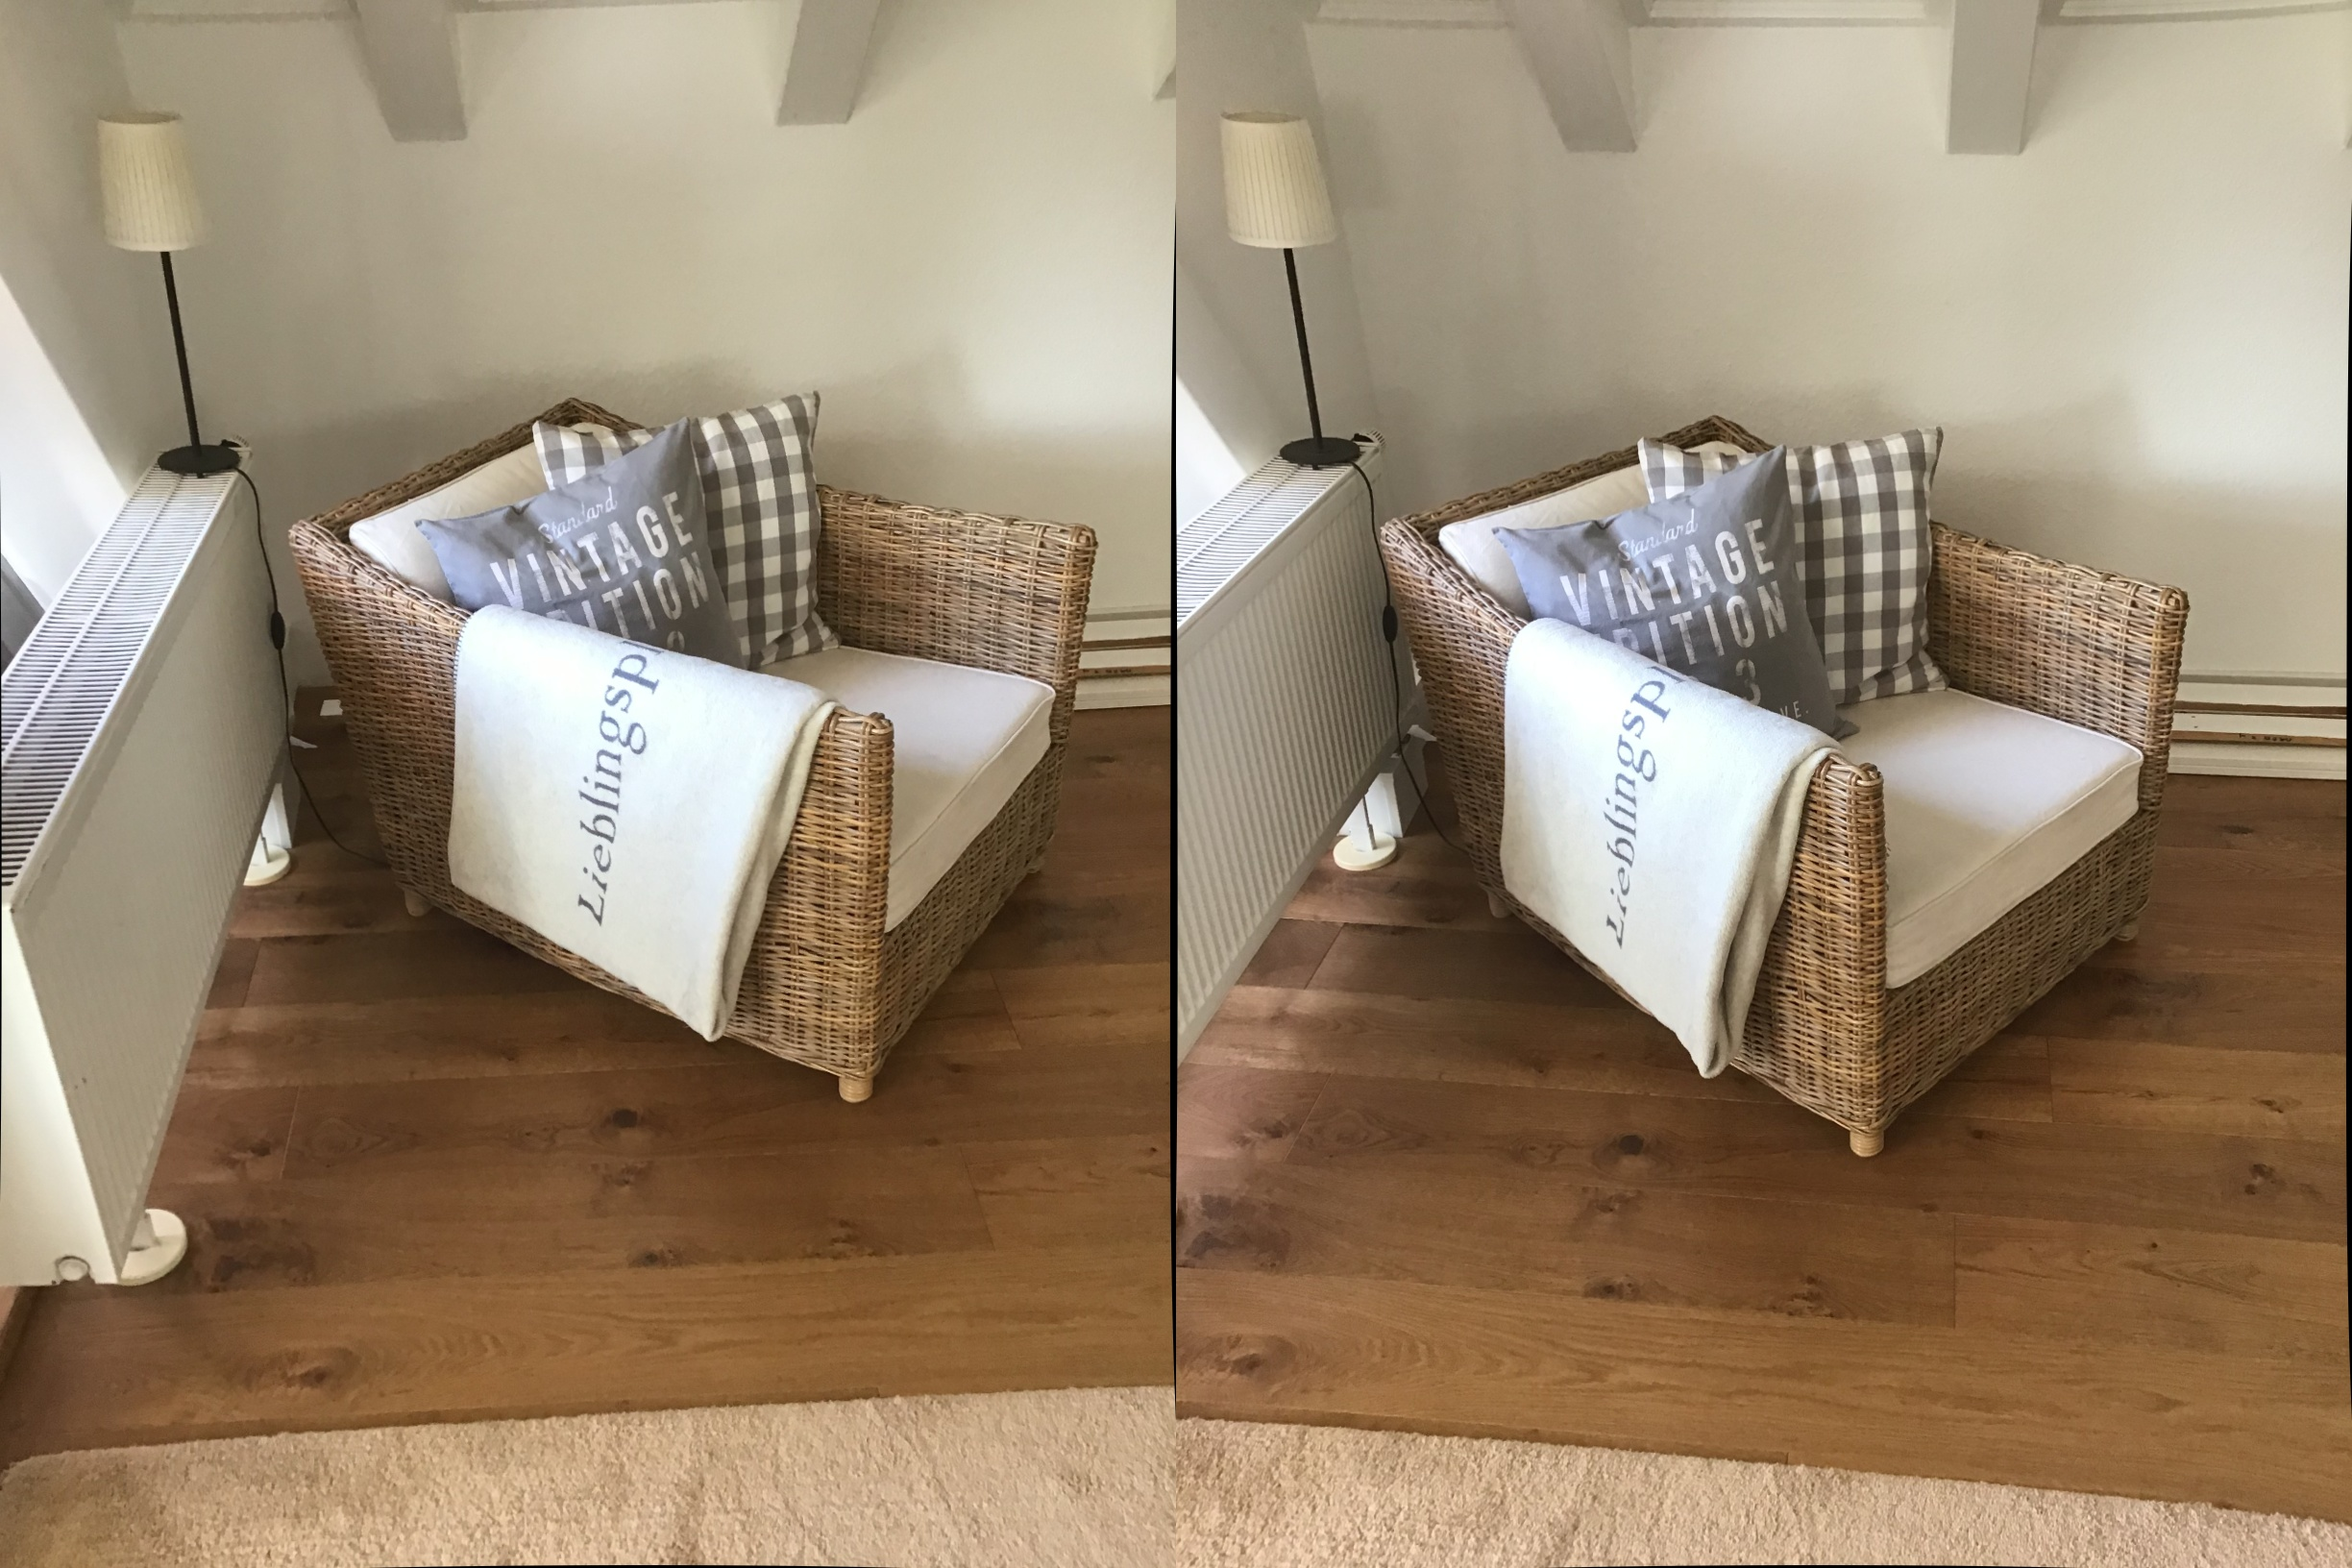
\includegraphics[width=\textwidth]{src/img/chair_first_pair.jpg}
    \caption{Eins von zehn Bildpaaren zum Rekonstruieren des Sessels.}
    \label{fig:chair-first-pair}
\end{figure}

\begin{figure}
    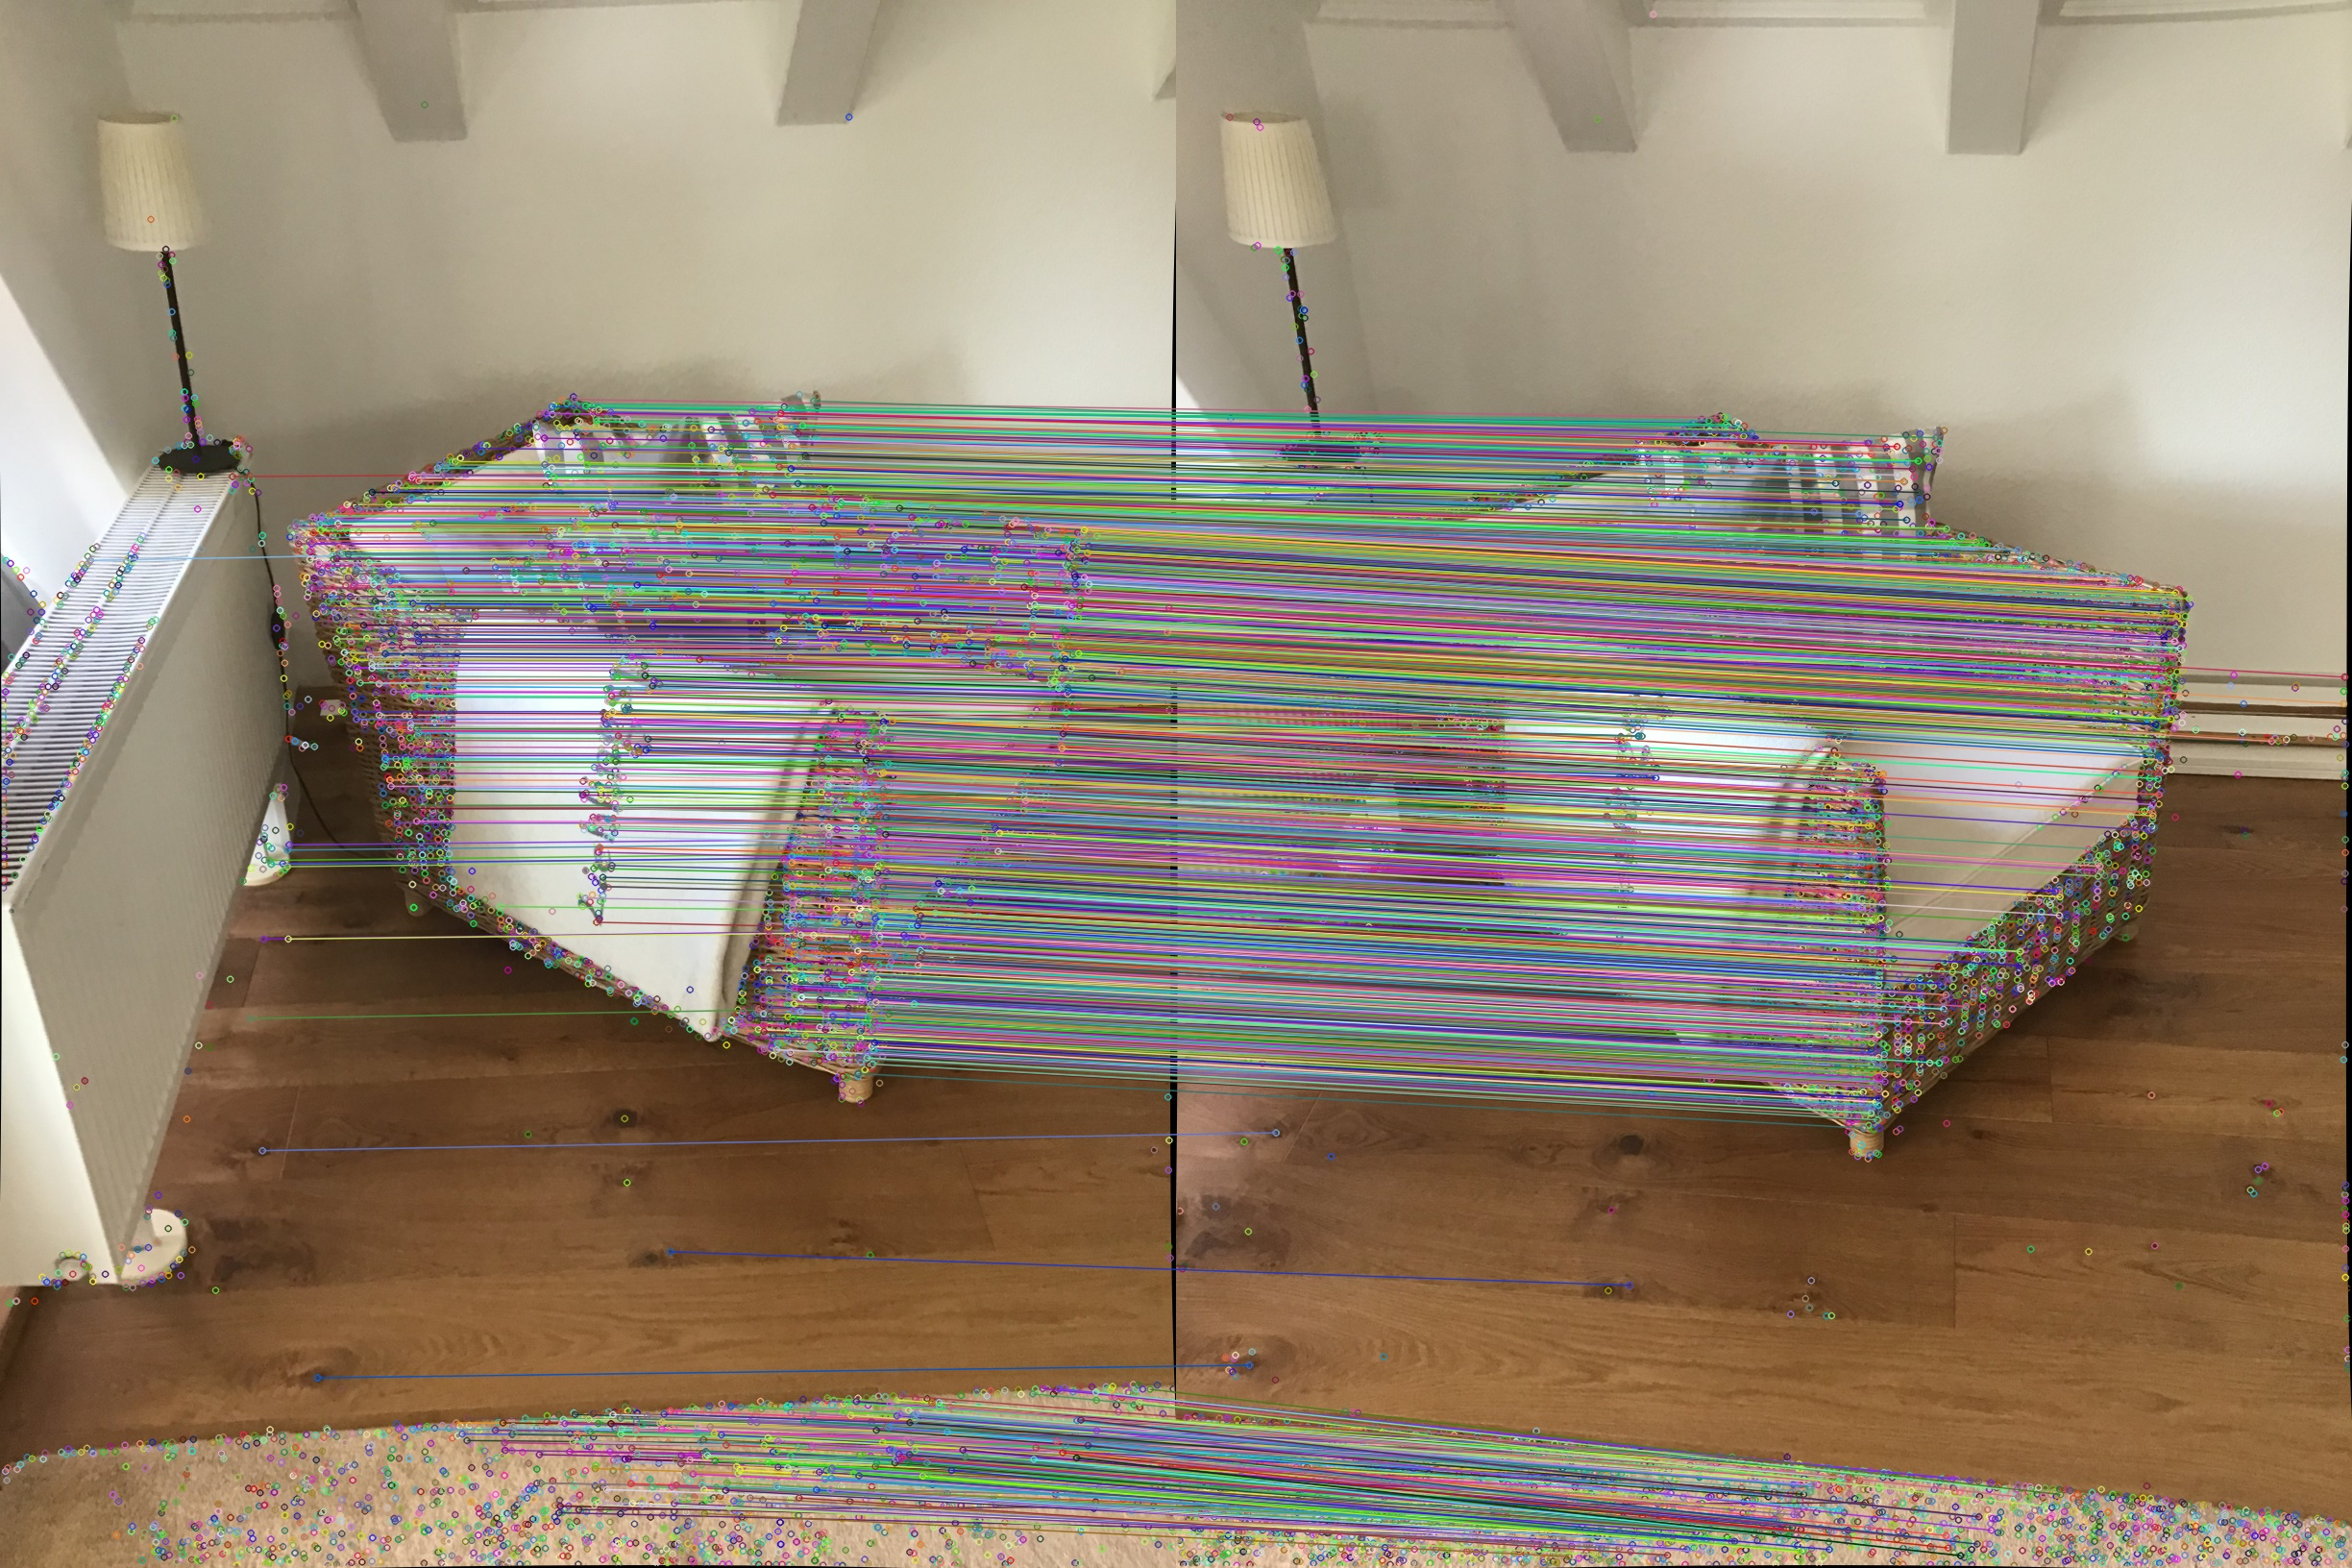
\includegraphics[width=\textwidth]{src/img/chair_first_pair_with_matches.jpg}
    \caption{Bildpaar des Sessels mit Keypoints und Matches.}
    \label{fig:chair-first-pair-with-matches}
\end{figure}

\begin{figure}
    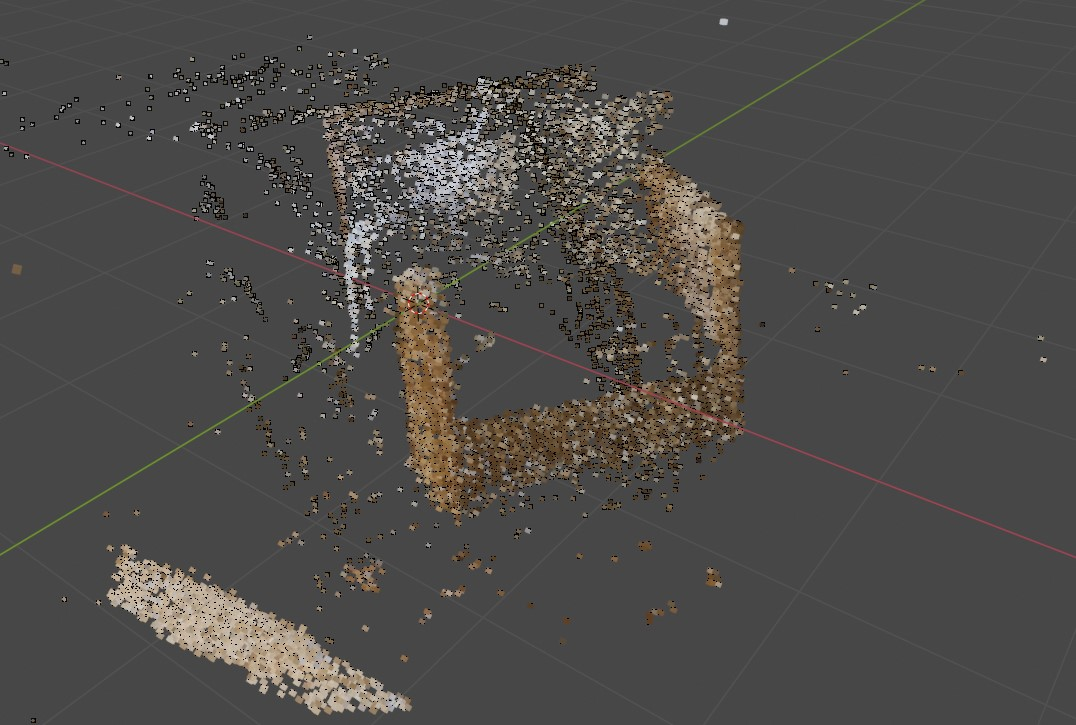
\includegraphics[width=\textwidth]{src/img/chair_model.jpg}
    \caption{Die rekonstruierten Bildpunkte des Sessels in Blender. Das Modell wurde um -119 Grad um die X gedreht, sowie um -4.8 Meter in Y und 2.7 Meter in Z Richtung verschoben.}
    \label{fig:chair-model}
\end{figure}

\begin{figure}
    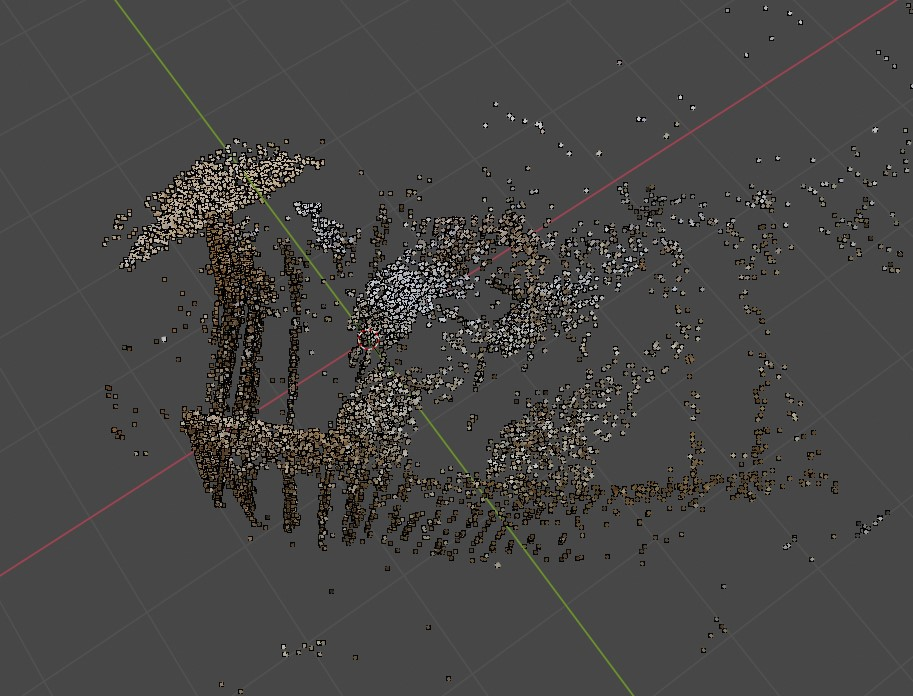
\includegraphics[width=\textwidth]{src/img/chair_model_2.jpg}
    \caption{Das Sessel Modell in einem anderem Blickwinkel}
    \label{fig:chair-model-2}
\end{figure}


\newpage
\section{Fall 2: Auto}
\label{sec:textcase-car}
Im zweiten Testfall wird die Rekonstruktion eines Autos getestet. 
Insgesamt wurden 17 Bilder von einem schwarzen Skoda Fabia gemacht, die das Auto in verschiedenen Positionen zeigt.
Die Tabelle~\cref{tab:car-results} zeigt Anzahl der rekonstruierten Punkte pro Bildpaar.
Im Vergleich zum ersten Testfall gibt es hier deutlich weniger Matches, rekonstruierte Punkte und Punkte,die für die Skalierung verwendet worden sind.
\cref{fig:car-second-pair,fig:car-second-pair-with-matches} zeigen das zweite Bildpaar vom Auto.
Hier ist sehen, dass dass die Keypoints der meisten Matches nicht auf auf dem Auto liegen.
Statt dessen werden Matches eher an den Wänden, Pflanzen und auf dem Boden gefunden.
Bei dem Auto selbst werden die Matches hauptsächlich nur am Nummernschild und vereinzelt in den Reflexionen der Umgebung gefunden.
Wie durch die schlechten Matches zu erwarten ist, kann das Auto in den rekonstruierten Modell nicht erkannt werden, wie in \cref{fig:car-model} zu sehen ist.
In \cref{fig:car-model-2} ist das Modell aus einem anderem Winkel zu sehen.
Hier ist deutlich zu erkennen, dass die grünen Punkte der Pflanzen im Hintergrund in der gleichen Ebene wie viele Andere Punkte liegen. 
Dies lässt auf einen Fehler in der Triangulation oder Skalierung der Punkte vermuten.

\begin{table}
    \begin{tabularx}{\textwidth}{c r r r r}
        \toprule
        Bildpaar &  Anzahl der Matches & Anzahl der Weltpunkte & Anzahl der Überlappende Weltpunkte & angewandte Skalierung \\ 
        \midrule
        1  & 575 & 480 & -  & - \\
        2  & 910 & 860 & 165 & 0,468641 \\
        3  & 685 & 653 & 227 & 0,768563 \\
        4  & 583 & 570 & 51  & 0,788242 \\
        5  & 264 & 247 & 25  & 0,60277 \\
        6  & 427 & 409 & 58  & 0,848896 \\
        7  & 393 & 346 & 95  & 2,80038 \\
        8  & 799 & 527 & 99  & 0,923119 \\
        9  & 827 & 518 & 113 & 0,577807 \\
        10 & 618 & 597 & 125 & 1,11263 \\
        11 & 251 & 187 & 56  & 0,472208 \\
        12 & 68  & 36  & 10  & 1,49154 \\
        13 & 341 & 325 & 2   & 1,33112 \\
        14 & 334 & 263 & 18  & 2,02715 \\
        15 & 175 & 166 & 12  & 0,475839 \\
        16 & 167 & 146 & 21  & 0,651284 \\
        \midrule
        Summe & 7.417 & 6.330 & 1.077 & - \\
        \bottomrule
    \end{tabularx}
    \caption{Ergebnis der Rekonstruktion der Autobilder.}
    \label{tab:car-results}
\end{table}

\begin{figure}
    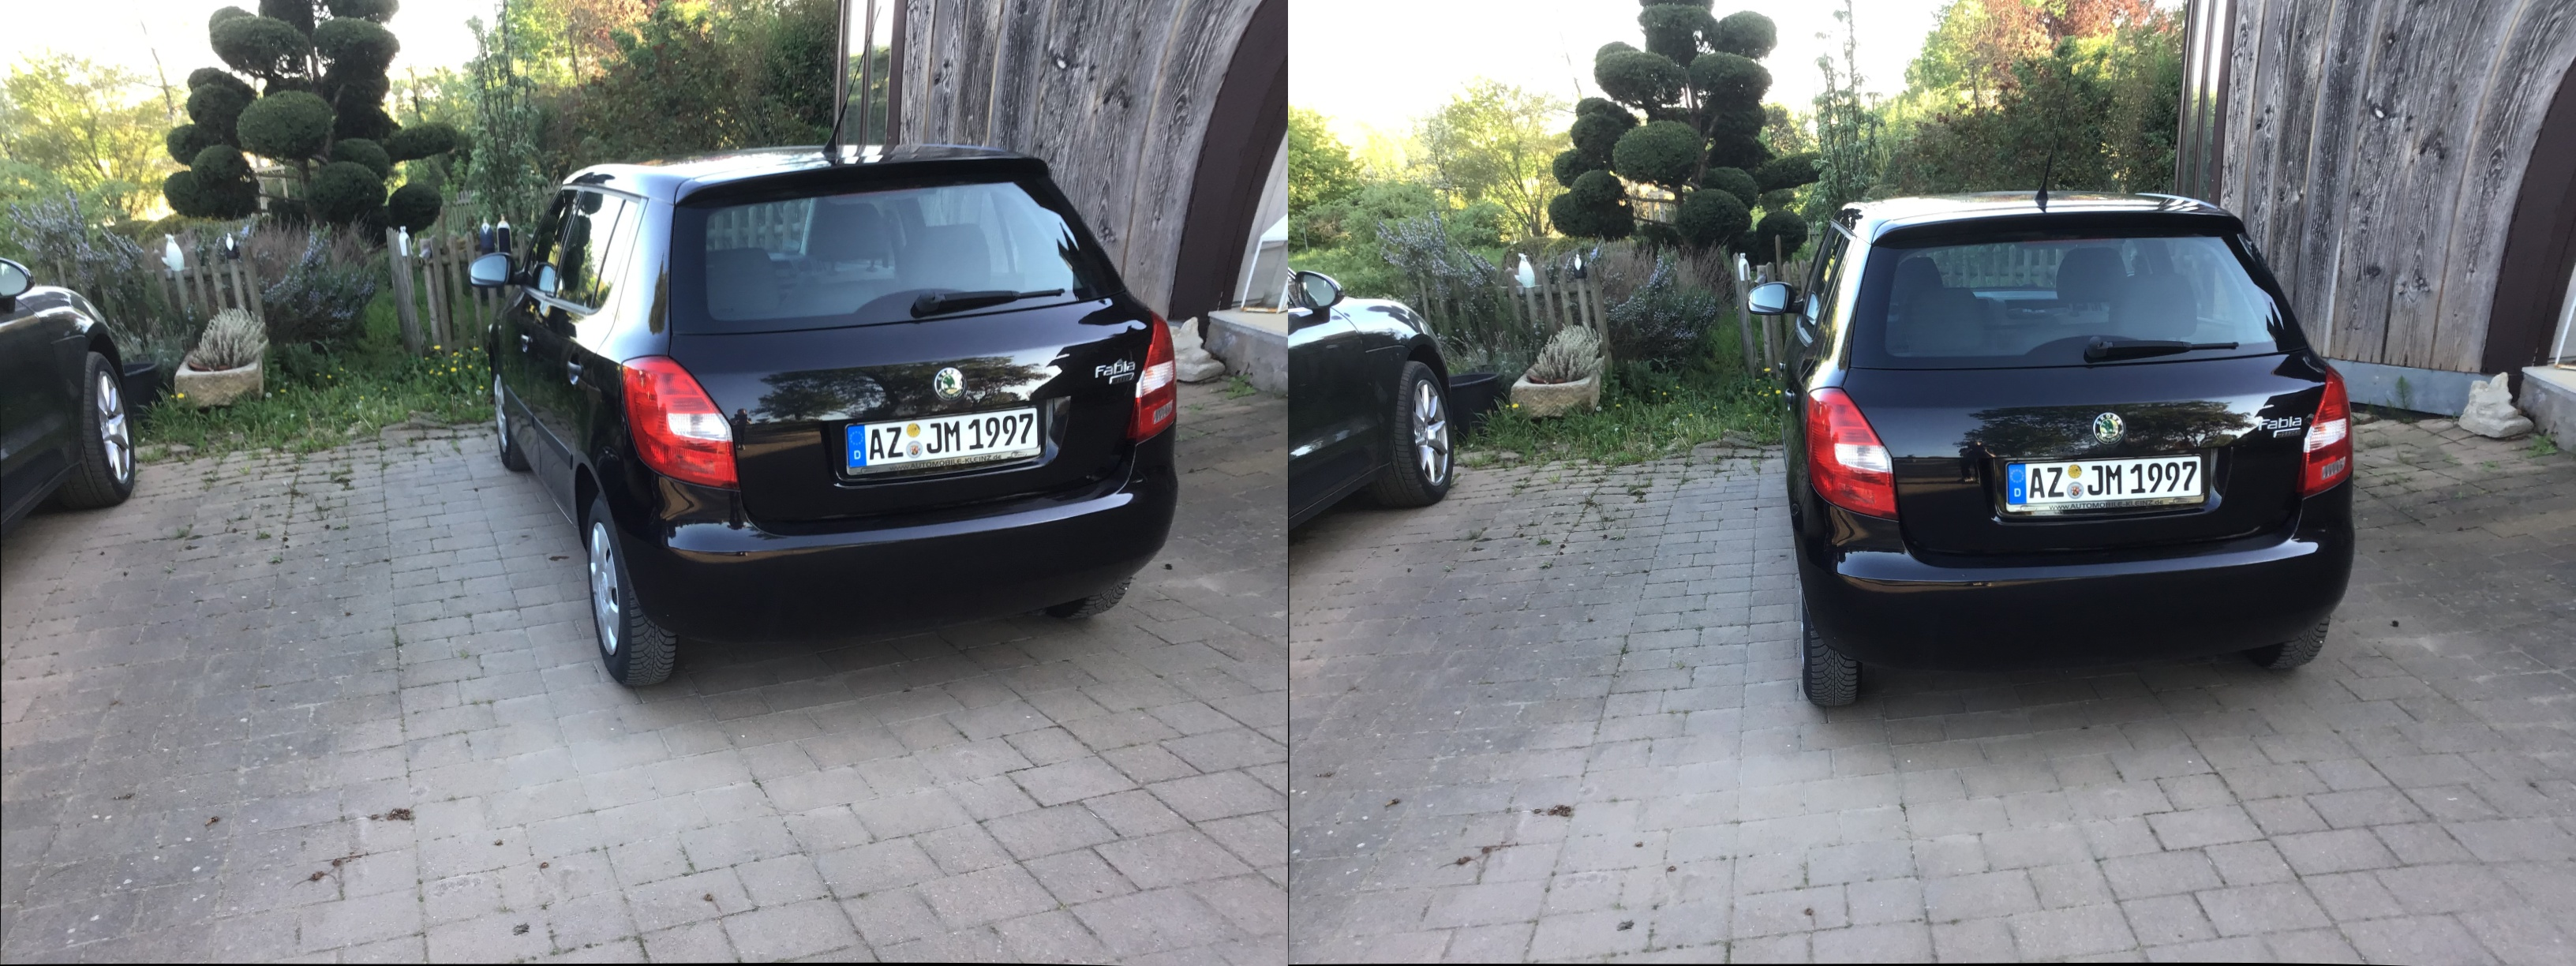
\includegraphics[width=\textwidth]{src/img/car_second_pair.jpg}
    \caption{Das zweite Bildpaar zum Rekonstruieren des Autos.}
    \label{fig:car-second-pair}
\end{figure}

\begin{figure}
    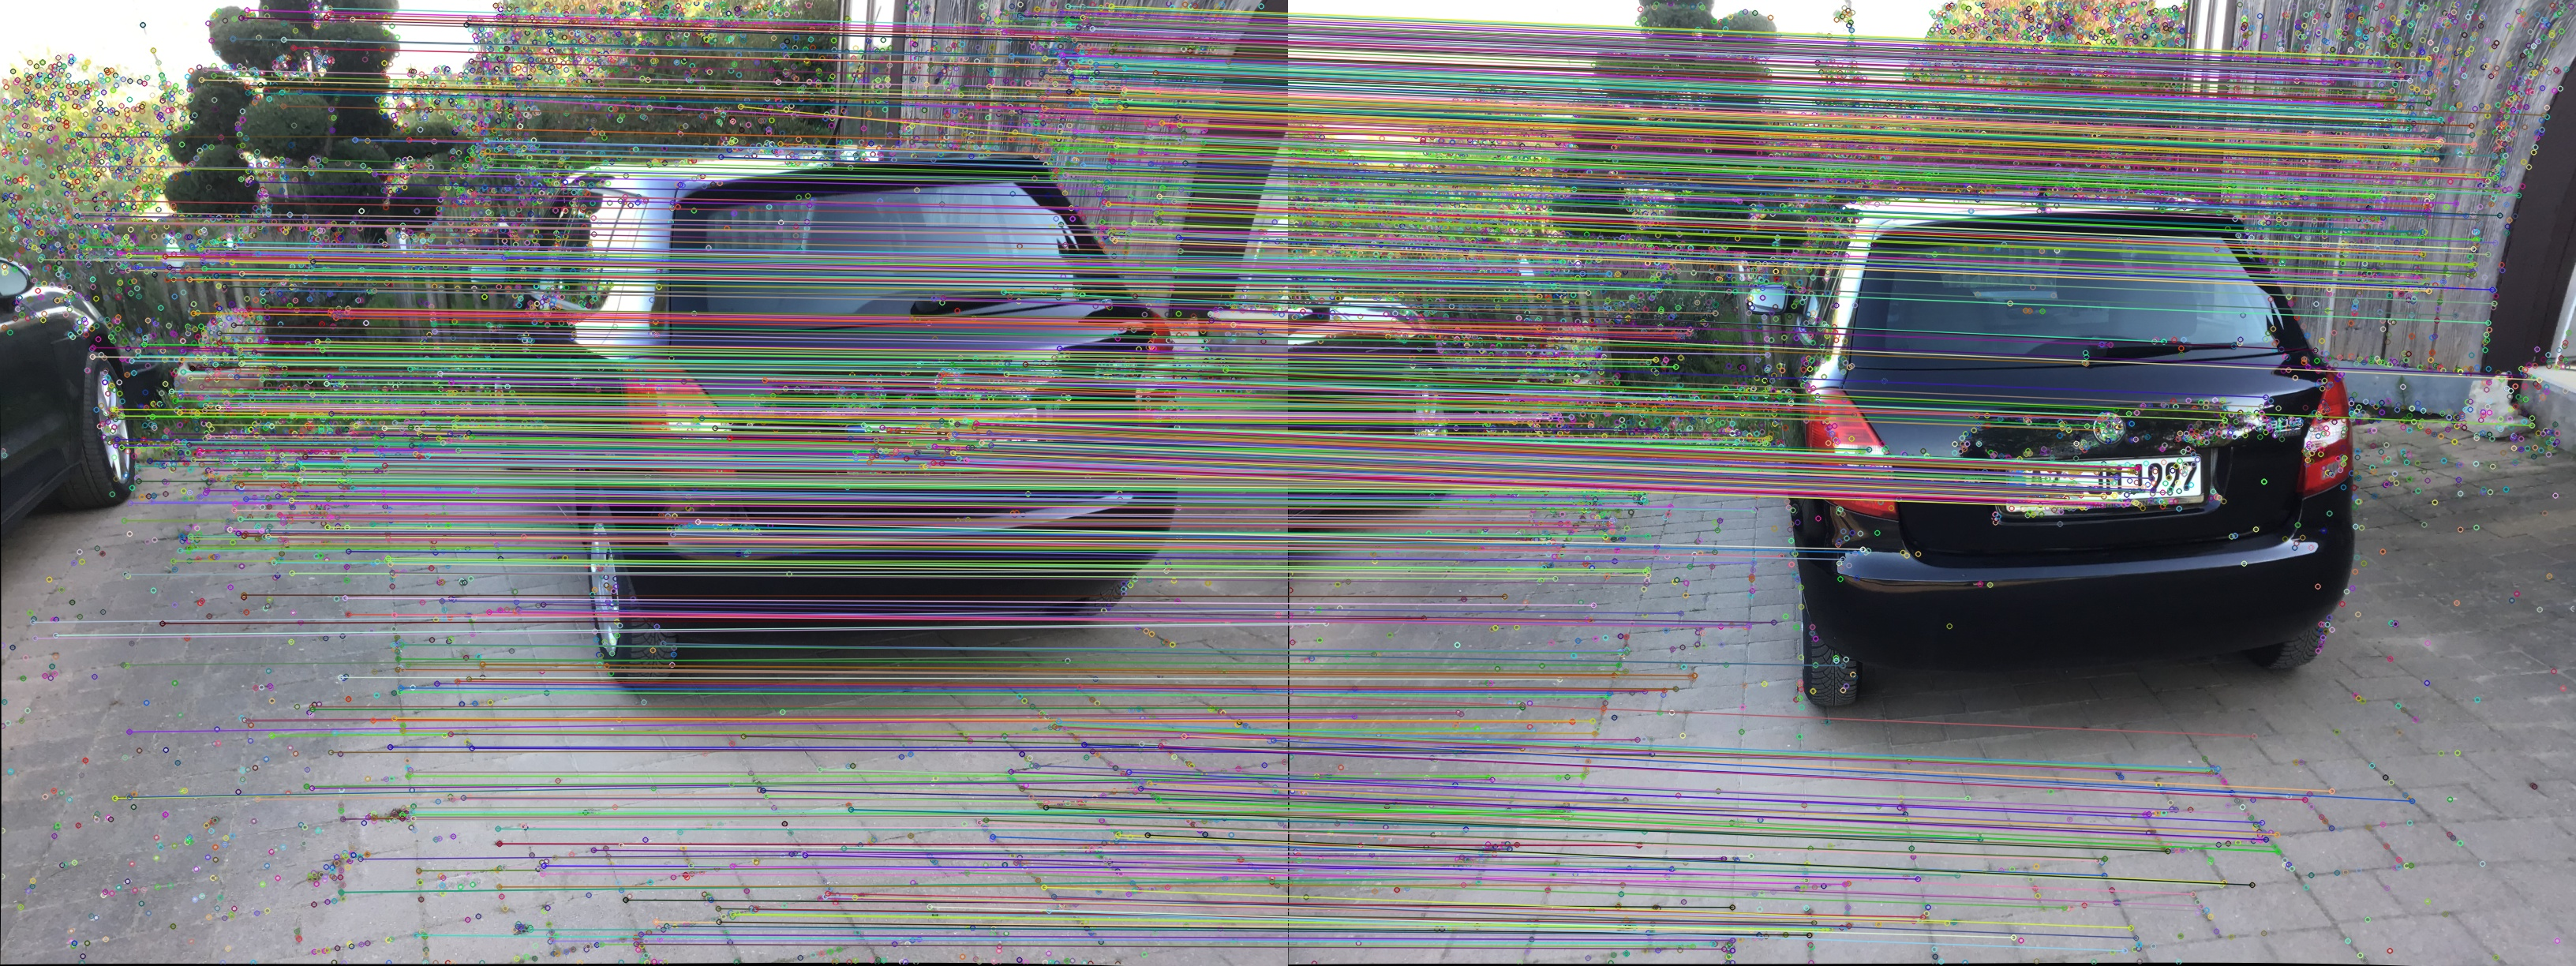
\includegraphics[width=\textwidth]{src/img/car_second_pair_with_matches.jpg}
    \caption{Das zweite Bildpaar vom Auto mit Keypoints und Matches.}
    \label{fig:car-second-pair-with-matches}
\end{figure}

\begin{figure}
    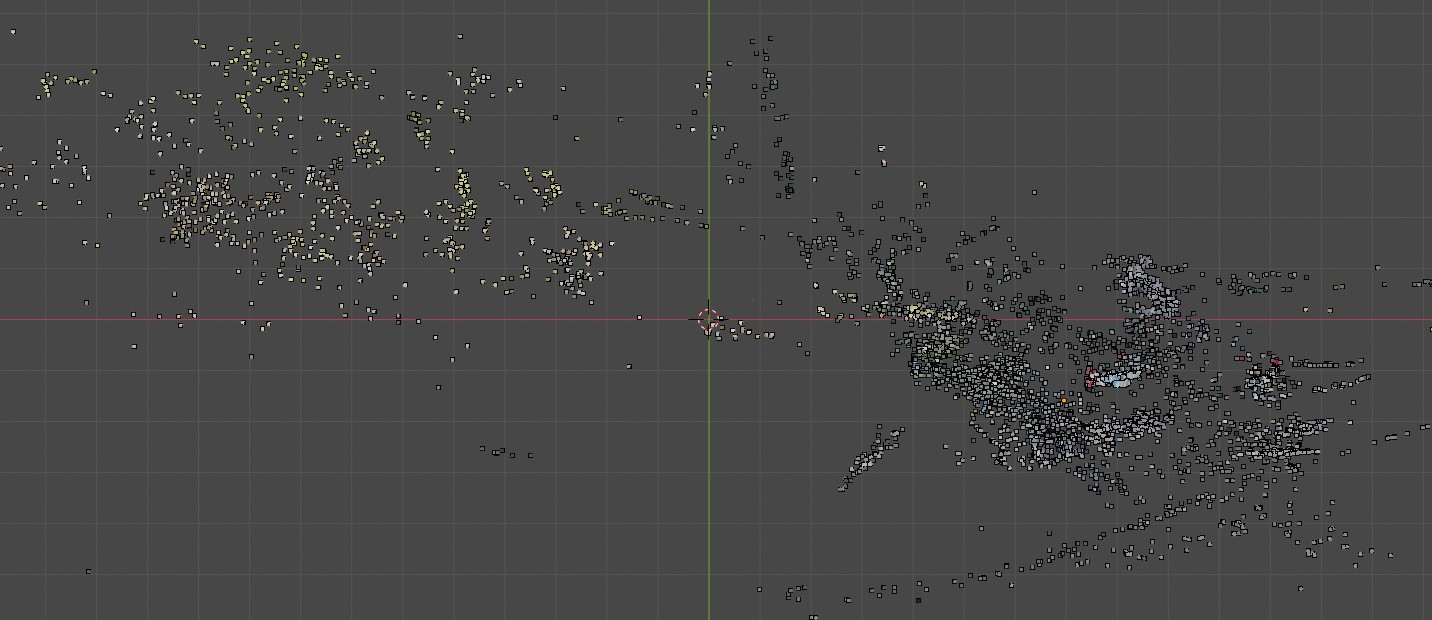
\includegraphics[width=\textwidth]{src/img/car_model.jpg}
    \caption{Das zweite Bildpaar vom Auto mit Keypoints und Matches.}
    \label{fig:car-model}
\end{figure}

\begin{figure}
    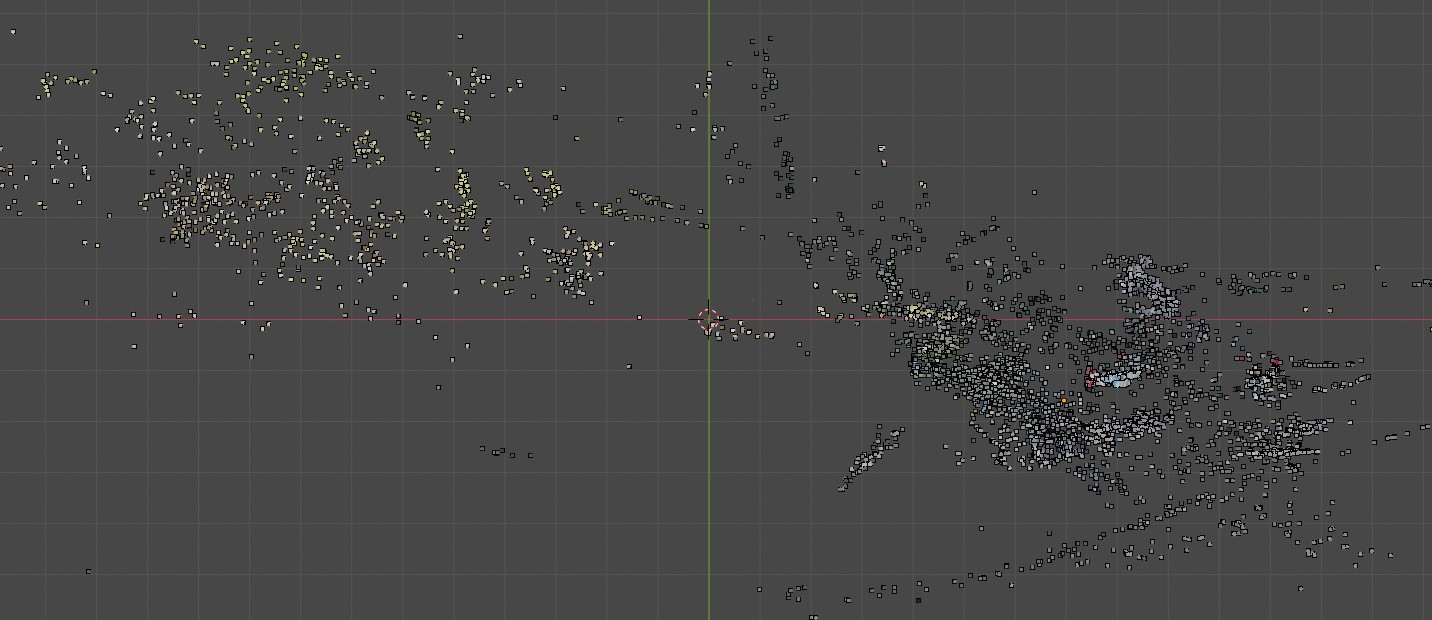
\includegraphics[width=\textwidth]{src/img/car_model.jpg}
    \caption{Das zweite Bildpaar vom Auto mit Keypoints und Matches.}
    \label{fig:car-model-2}
\end{figure}

\newpage
\section{Fall 3: Hund}
\label{sec:testcase-dog}
Im dritten Testfall wird versucht mit neuen Bildern einen Hund in einem Körbchen zu rekonstruieren, der in \cref{fig:dog-image} zu sehen ist.

Die \cref{tab:dog-results} zeigt die Ergebnisse der Rekonstruktion.
In allen Bildpaaren ist der Matches höher als im ersten Testfall.
Betracht man jedoch in \cref{fig:dog-first-pair-with-matches} wo die Matches liegen, dann fällt auf, dass keine auf dem Hund liegen.
Stattdessen befinden sich alle Matches auf dem Teppich.
Das Modell in Blender zeigt dem entsprechend nur eine Fläche, die aus beige Punkten besteht.
Das Problem in diesem Testfall ist wie beim Auto und dem Sitzkissen des Sessels, dass der Hund keine auffälligen Kanten besitzt, die als Feature erkannt werden.
Des Weiteren ist das Aufnehmen der Fotos in diesem Fall problematisch. 
Im Vergleich zum Sessel oder dem Auto ist es schwierig mehrere und gute Bilder von dem Hund zu machen, ohne dass er sich bewegt. 
Es war nicht möglich den Hund stehend zu fotografieren, da er entweder weiter gelaufen ist oder den Kopf mit der Kamera bewegt hat.
Die Fotos konnten erst dann gemacht werden, wenn der Hund zufällig im Körbchen gelegen hat und sich nicht beweg hat.

\begin{figure}
    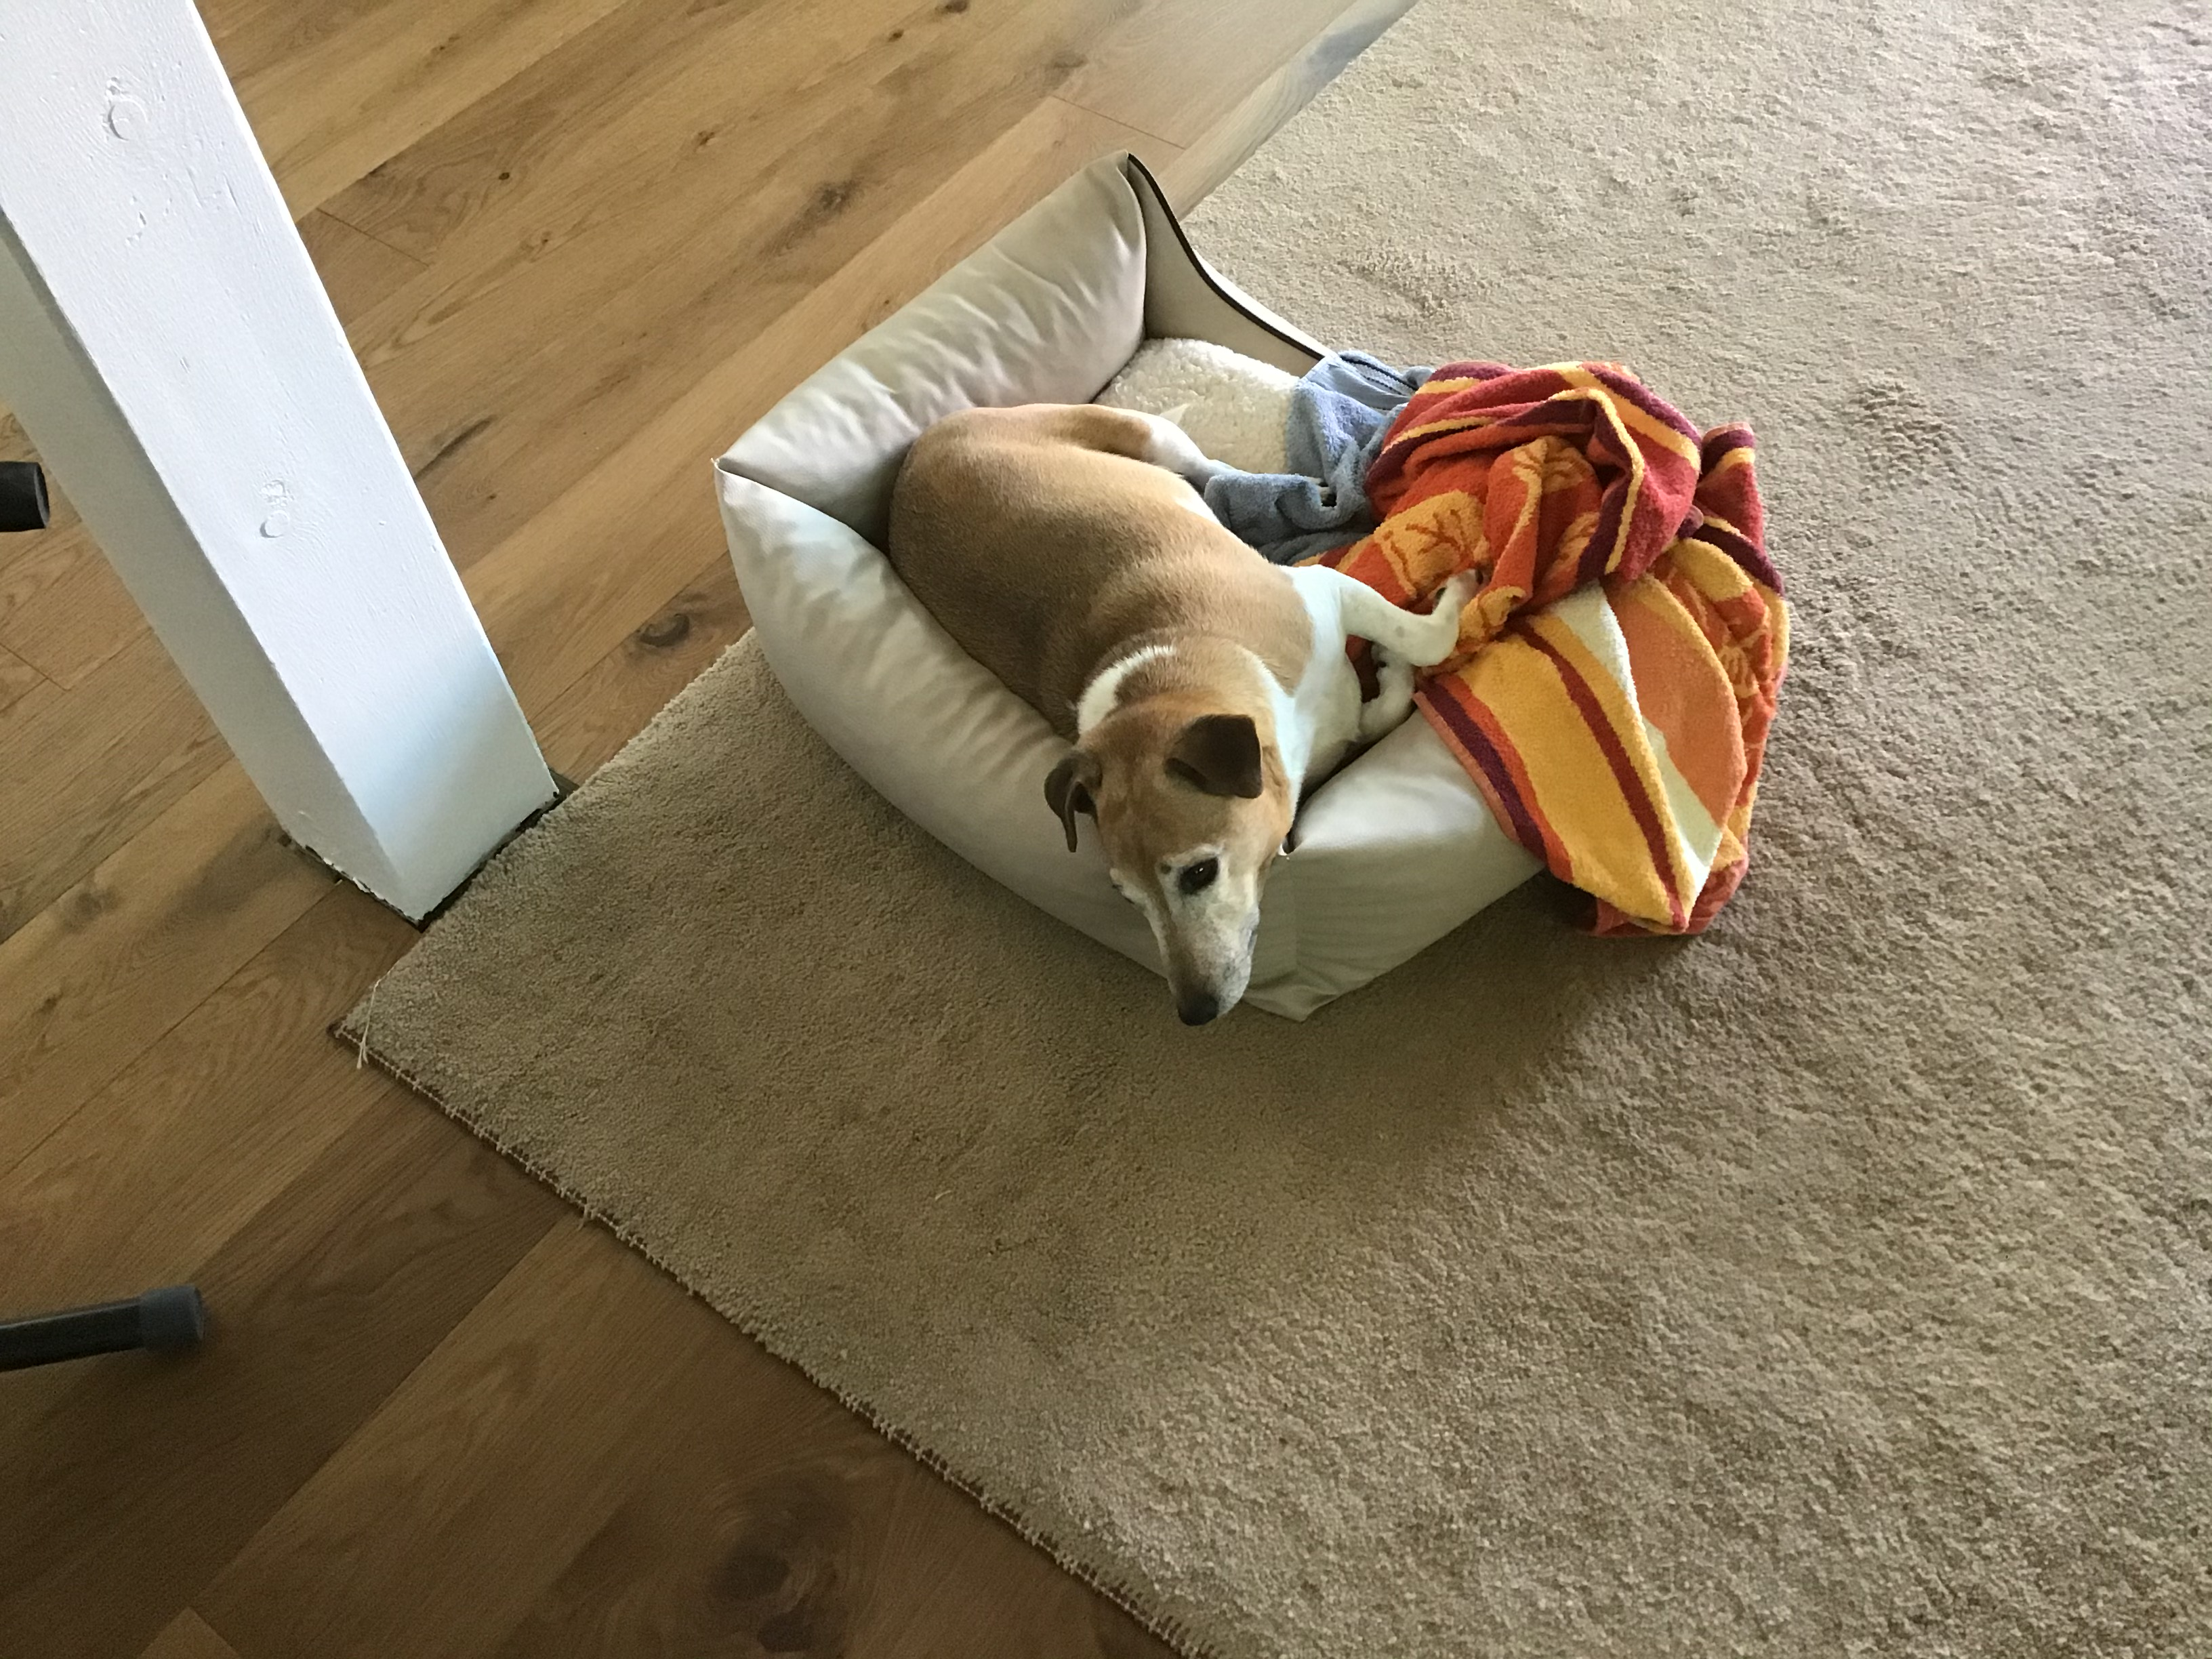
\includegraphics[width=\textwidth]{src/img/dog.jpg}
    \caption{Der Hund, genannt Sam, der im Körbchen liegt und rekonstruiert wird.}
    \label{fig:dog-image}
\end{figure}

\begin{table}
    \begin{tabularx}{\textwidth}{cXXXX}
        \toprule
        Bildpaar &  Anzahl der Matches & Anzahl der Weltpunkte & Anzahl der Weltpunkte für Skalierung & angewandte Skalierung \\ 
        \midrule
        1 & 4.799 & 4.786 & -  & - \\
        2 & 6.450 & 6.421 & 2.127 & 0,835131 \\
        3 & 6.525 & 6.472 & 2.763 & 0,892978 \\
        4 & 7.520 & 7.489 & 2.867 & 0,975344 \\
        5 & 7.462 & 7.444 & 3.215 & 0,801014 \\
        6 & 3.024 & 2.984 & 1.651 & 0,93856  \\
        7 & 6.071 & 6.009 & 1.337 & 1,42251  \\
        8 & 7.893 & 7.874 & 3.091 & 0,707064 \\
        9 & 6.917 & 4.350 & 1.924 & 1,01307  \\
        \midrule
        Summe & 56.661 & 53.829 & 18.975 & - \\
        \bottomrule
    \end{tabularx}
    \caption{Ergebnis der Rekonstruktion der neun Hundebilder}
    \label{tab:dog-results}
\end{table}

\begin{figure}
    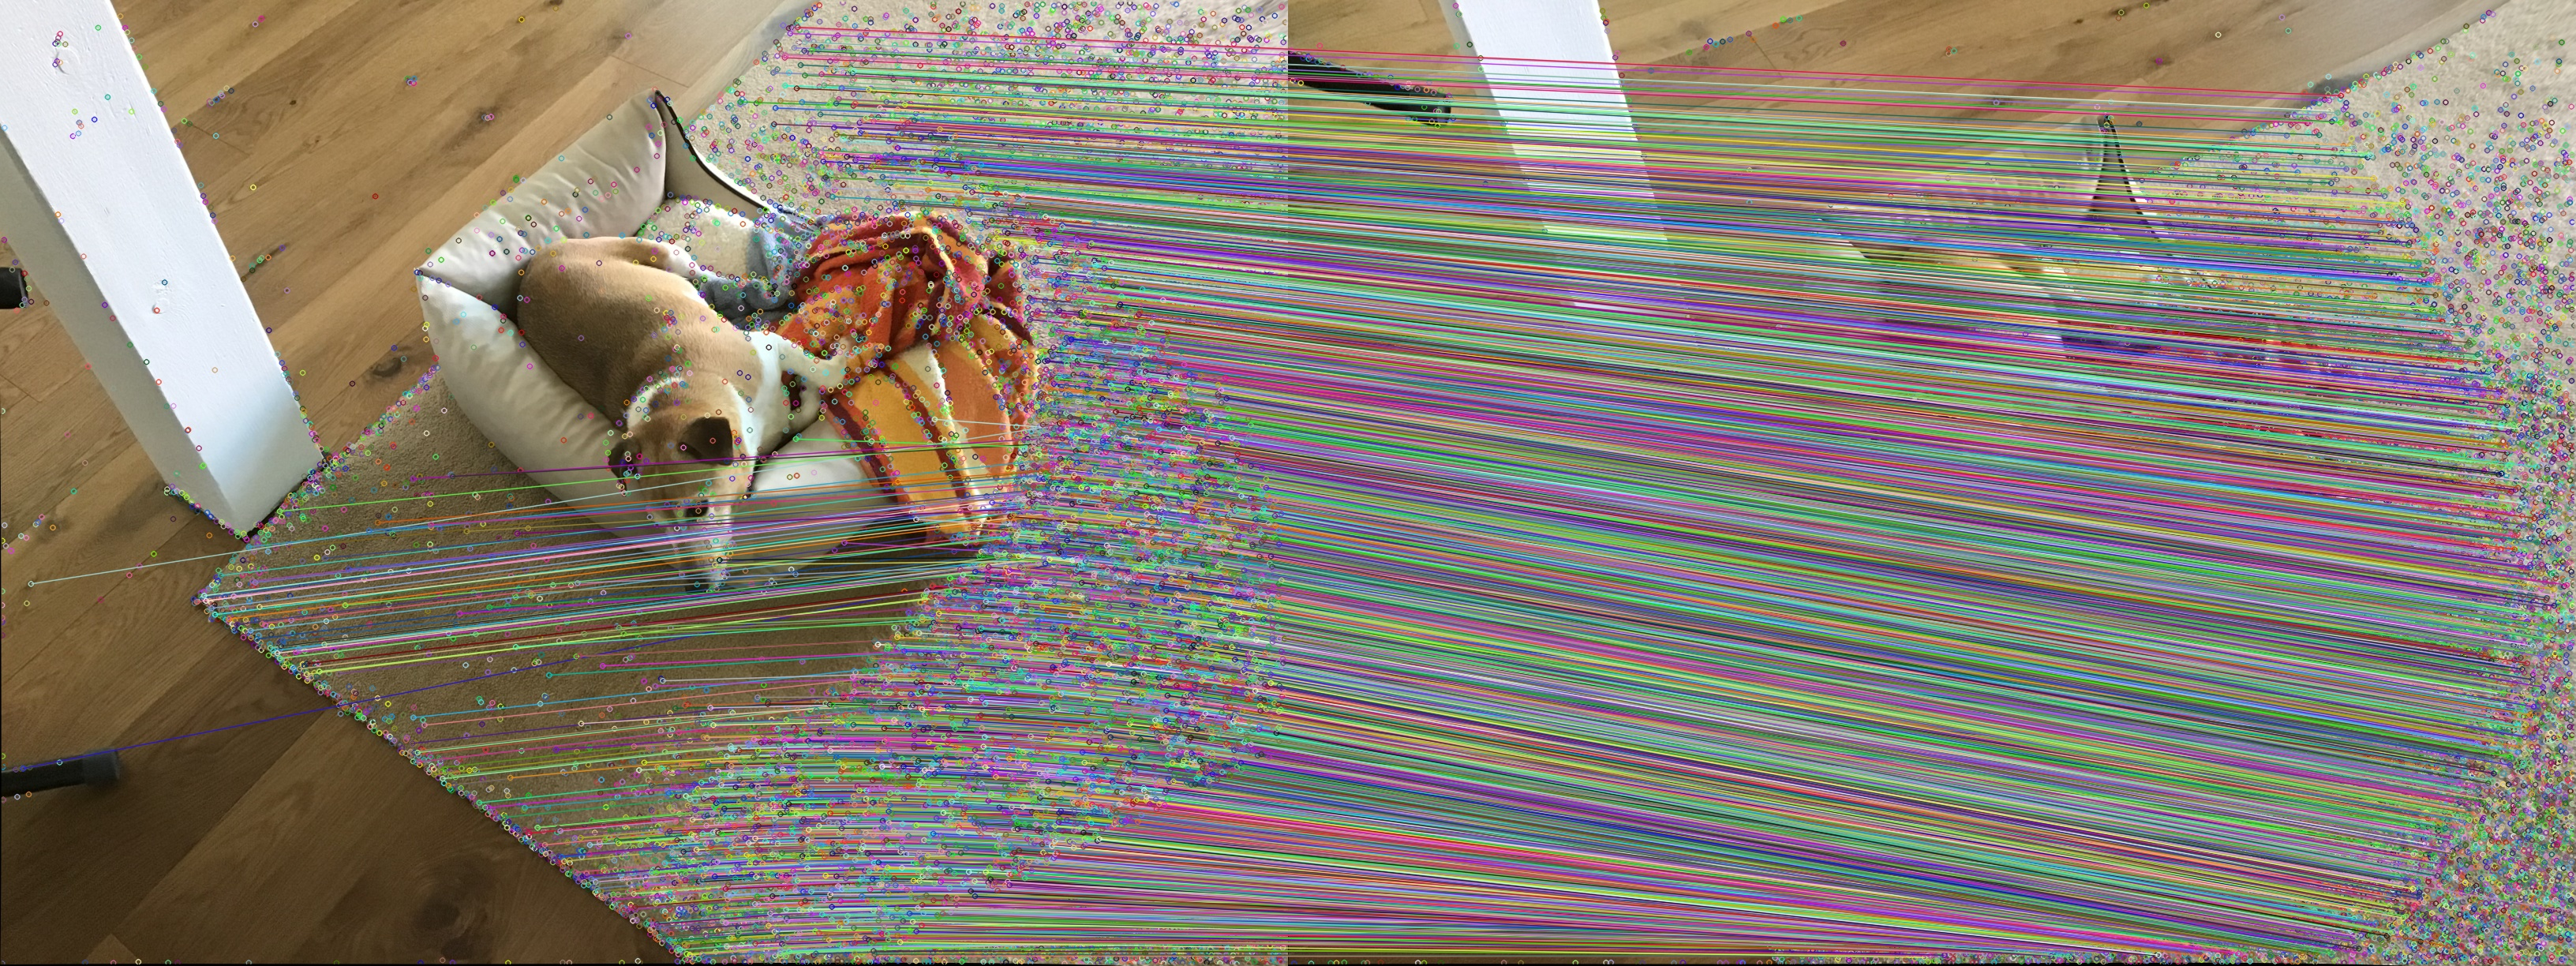
\includegraphics[width=\textwidth]{src/img/dog_first_pair_with_matches.jpg}
    \caption{Das erste der neun 8 Bildpaare, das die Keypoints und ihre Matches zeigt.}
    \label{fig:dog-first-pair-with-matches}
\end{figure}

\begin{figure}
    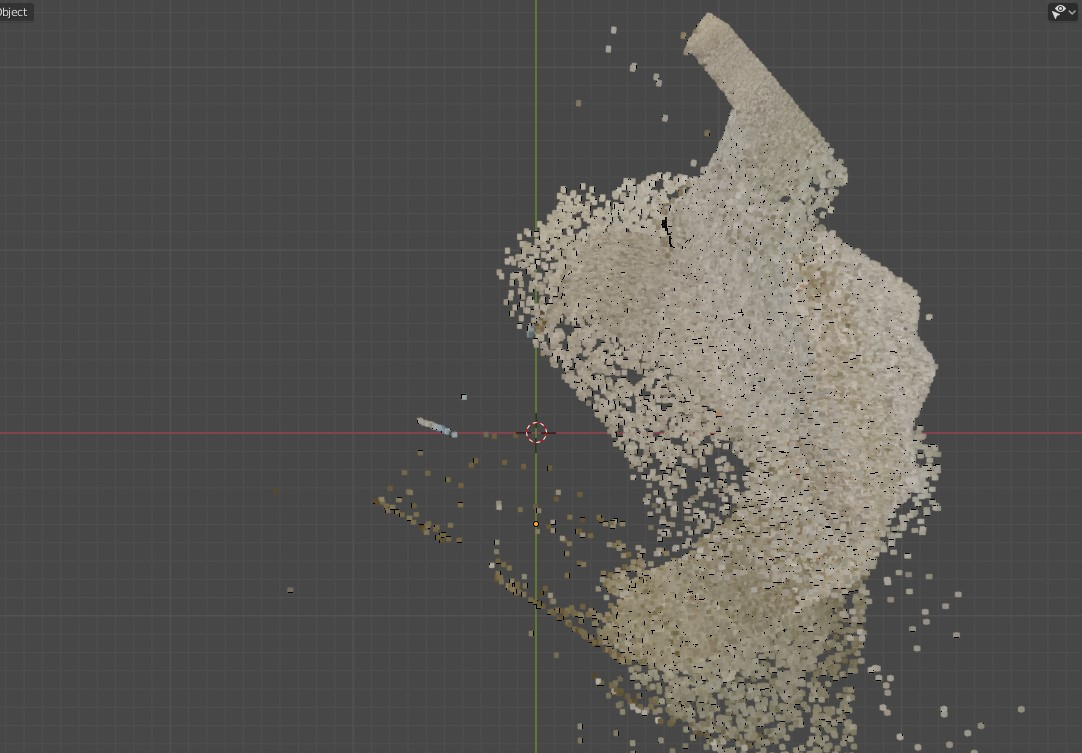
\includegraphics[width=\textwidth]{src/img/dog_model.jpg}
    \caption{Die rekonstruierten Punkte aus den Hundebildern. Das Bild zeigt das Modell ungefähr aus der Position der ersten Kamera.}
    \label{fig:dog-model}
\end{figure}

\begin{figure}
    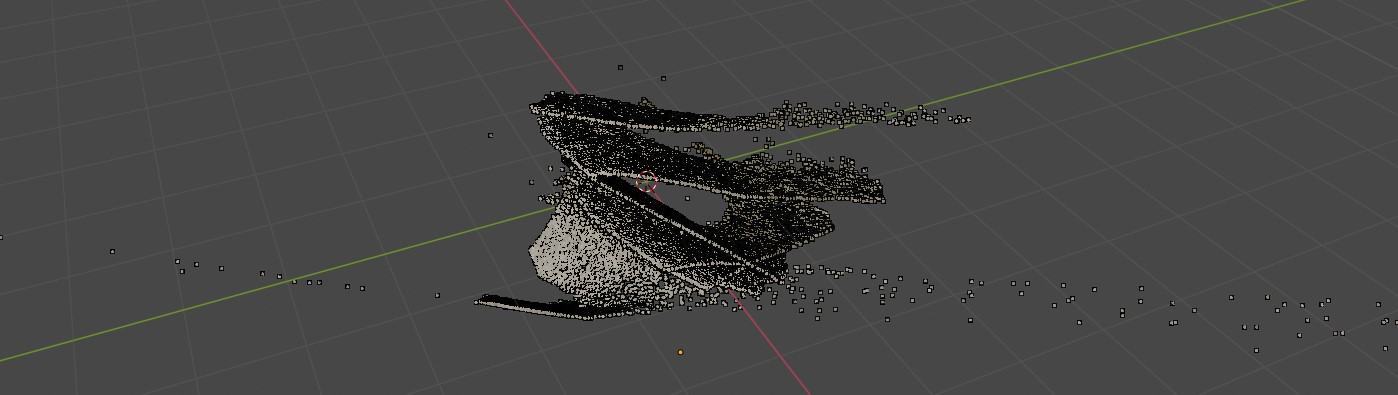
\includegraphics[width=\textwidth]{src/img/dog_model_2.jpg}
    \caption{Die rekonstruierten Punkte aus den Hundebildern. Das Bild zeigt das Modell von der Seite.}
    \label{fig:dog-model-2}
\end{figure}

\newpage
\section{Fall 4: Box}
\label{sec:testcase-box}\ohead{Sebastian Schmitt}
Im vierten Testfall wird versucht eine Box anhand von fünf Bildern zu rekonstruieren.
Diese ist in \autoref{fig:box-image} zu sehen.

Die \autoref{tab:box-results} zeigt die Ergebnisse der Rekonstruktion.
Es fällt auf, dass nur vergleichsweise sehr wenige Matches gefunden werden.
Betracht man jedoch in \autoref{fig:box-first-pair-with-matches} wo Keypoints und Matches liegen, erkennt man, dass die meisten Matches durchaus direkt an der Box bzw. an dem Kissen auf der Box gefunden wurden.
Besonders das Kissen und die Vorderseite der Box kann man in \autoref{fig:box-model} gut erkennen.
Diese guten Matches kommen zustande, da es in den Bildern klare Flächen mit identifizierbaren Kanten gibt.
Dass auf der Seite der Box keine Matches gefunden wurden, ist dadurch zu erklären, dass jeweils nur ein Bild existiert auf welchem eine Boxseite zu erkennen ist.
Betrachtet man \autoref{fig:box-model-2}, so erkennt man etwas oberhalb deutlich weitere Punkte zu Kissen bzw. Boxdeckel, welche eigentlich tiefer liegen müssten.
Dies lässt ähnlich wie in \autoref{sec:textcase-chair} eine ungenaue Skalierung des Translationsvektors vermuten.

\begin{figure}
    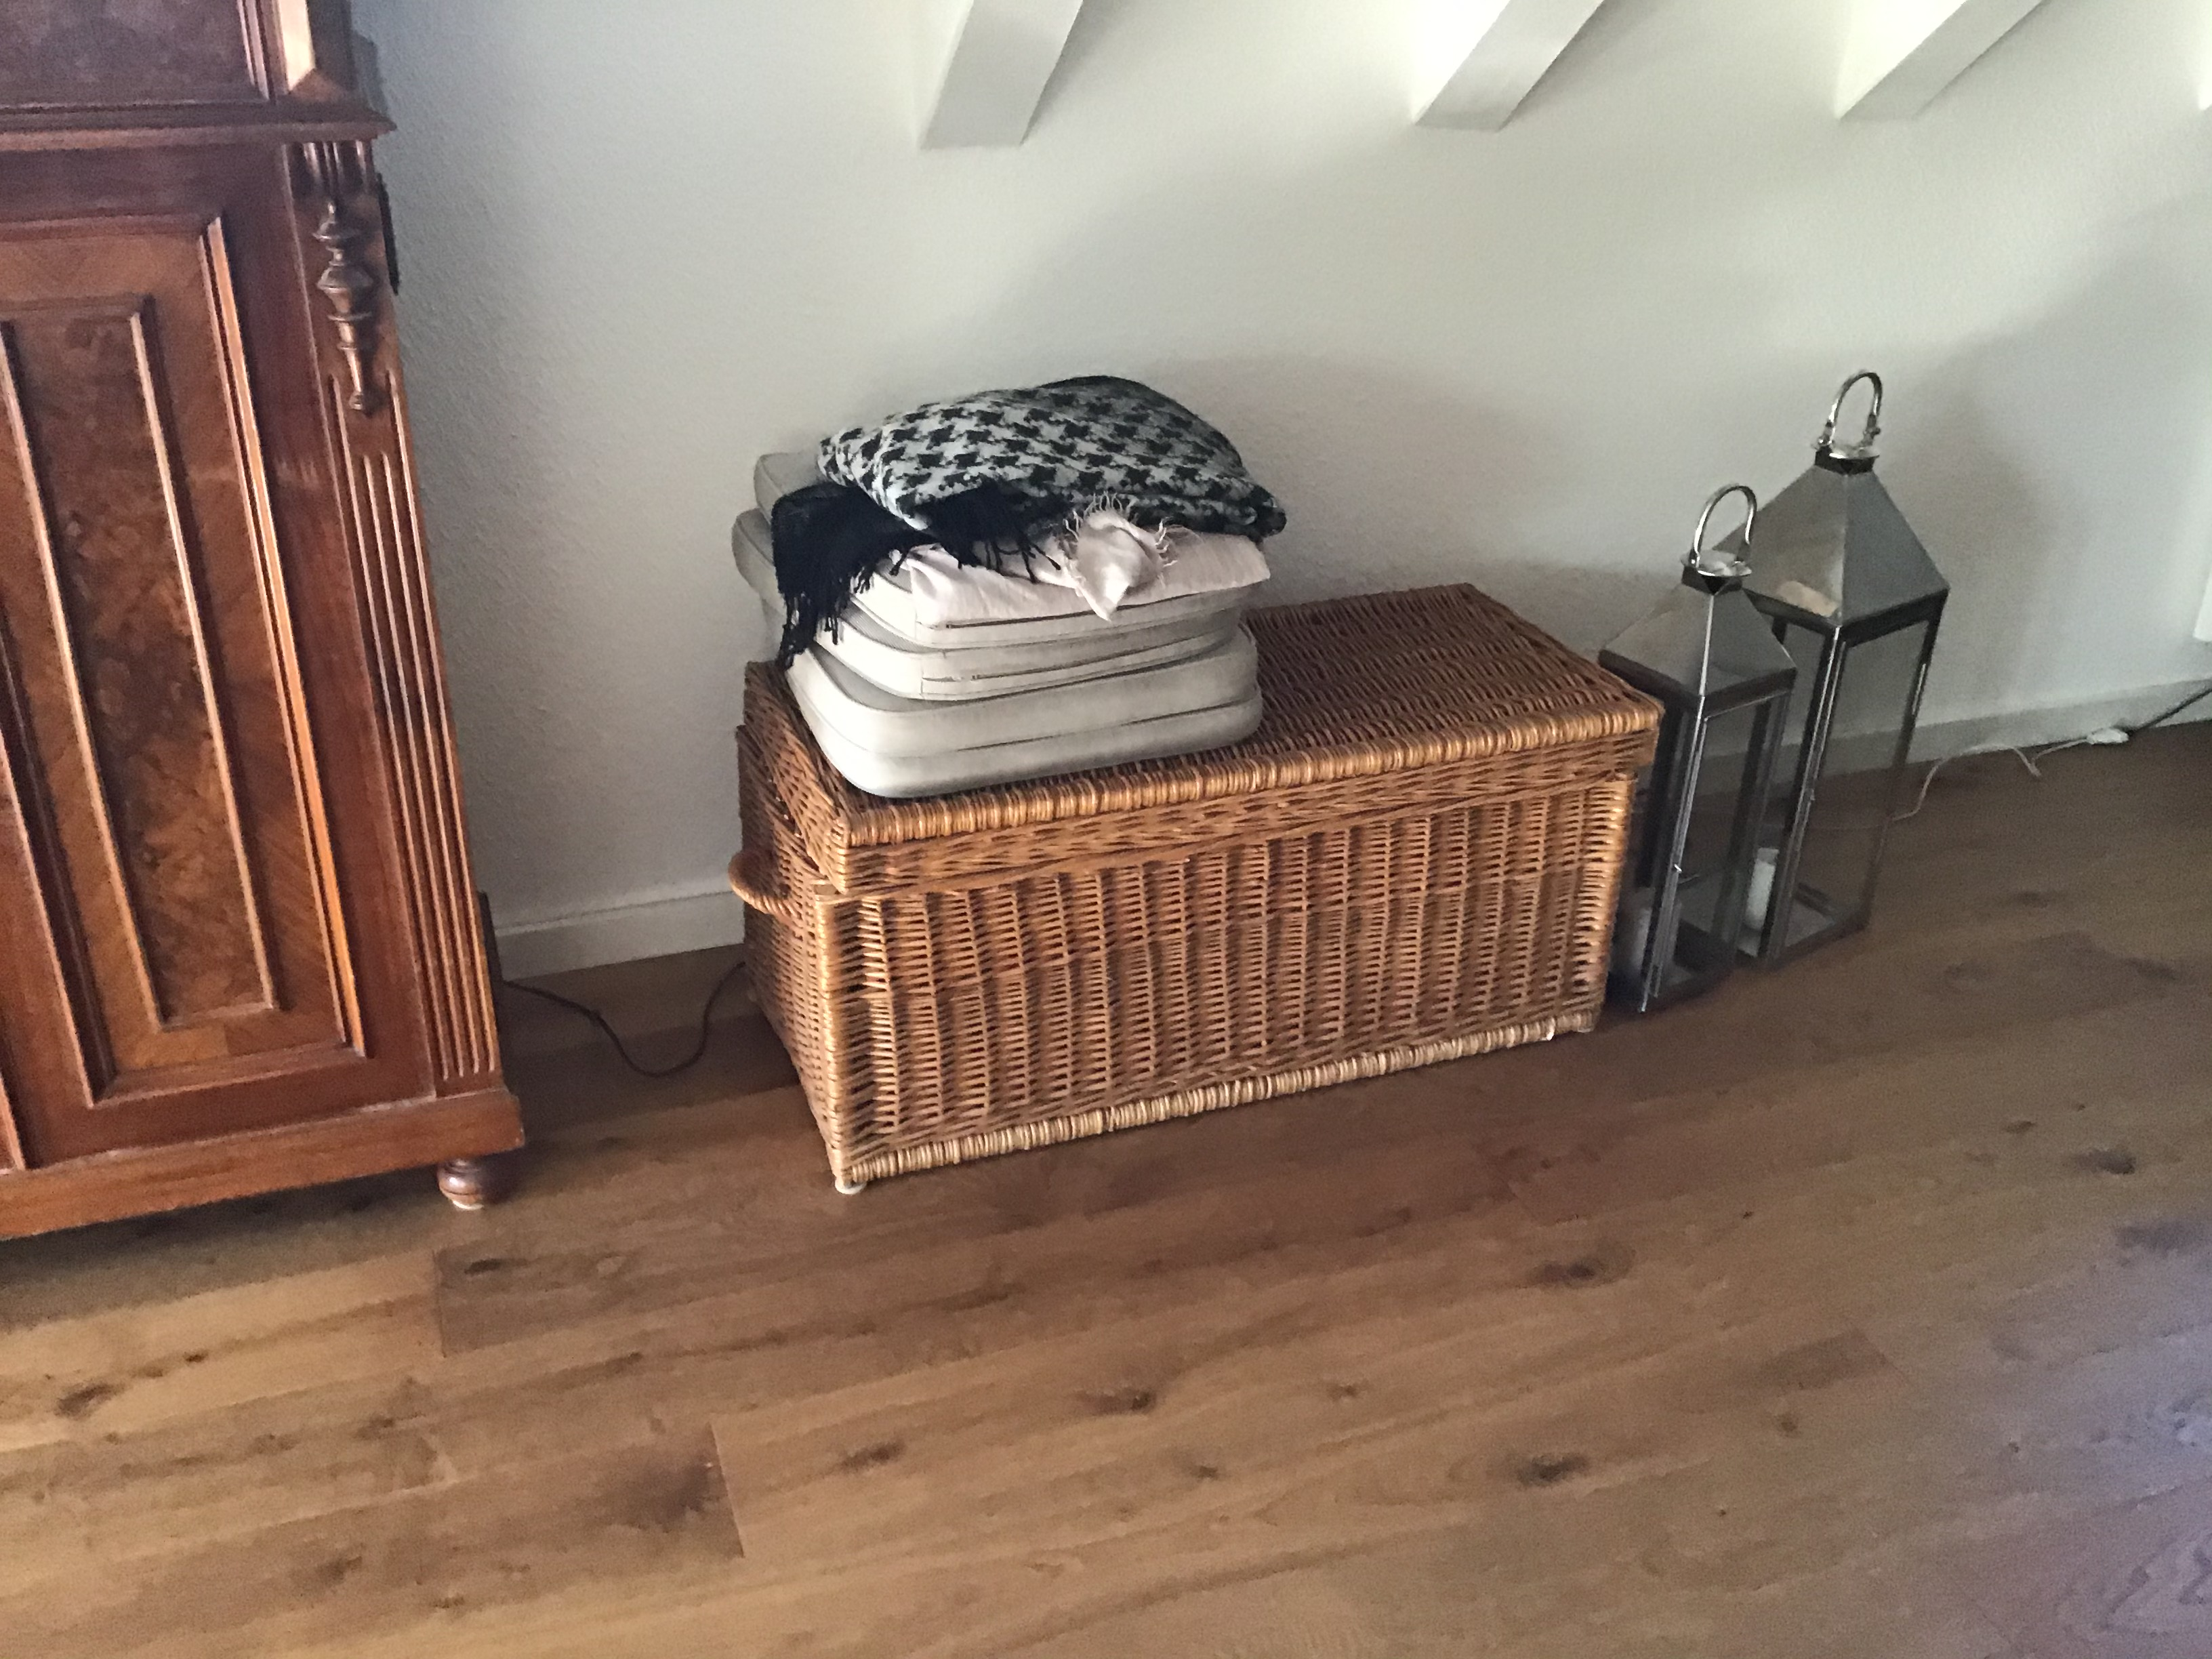
\includegraphics[width=\textwidth]{src/img/box.jpg}
    \caption{Die Box welche rekonstruiert wird}
    \label{fig:box-image}
\end{figure}

\begin{table}
    \begin{tabularx}{\textwidth}{XXXXX}
        \toprule
        Bildpaar &  Anzahl der Matches & Anzahl der Weltpunkte & Anzahl der überlappenden Weltpunkte & angewandte Skalierung \\ 
        \midrule
        1 & 267 & 215 & -  & - \\
        2 & 914 & 215 & 81 & 0,667182 \\
        3 & 433 & 359 & 117 & 1,34628 \\
        4 & 1.170 & 1.154 & 131 & 0,542451 \\
        \midrule
        Summe & 2.786 & 2.542 & 329 & - \\
        \bottomrule
    \end{tabularx}
    \caption{Ergebnis der Rekonstruktion der neun Hundebilder}
    \label{tab:box-results}
\end{table}

\begin{figure}
    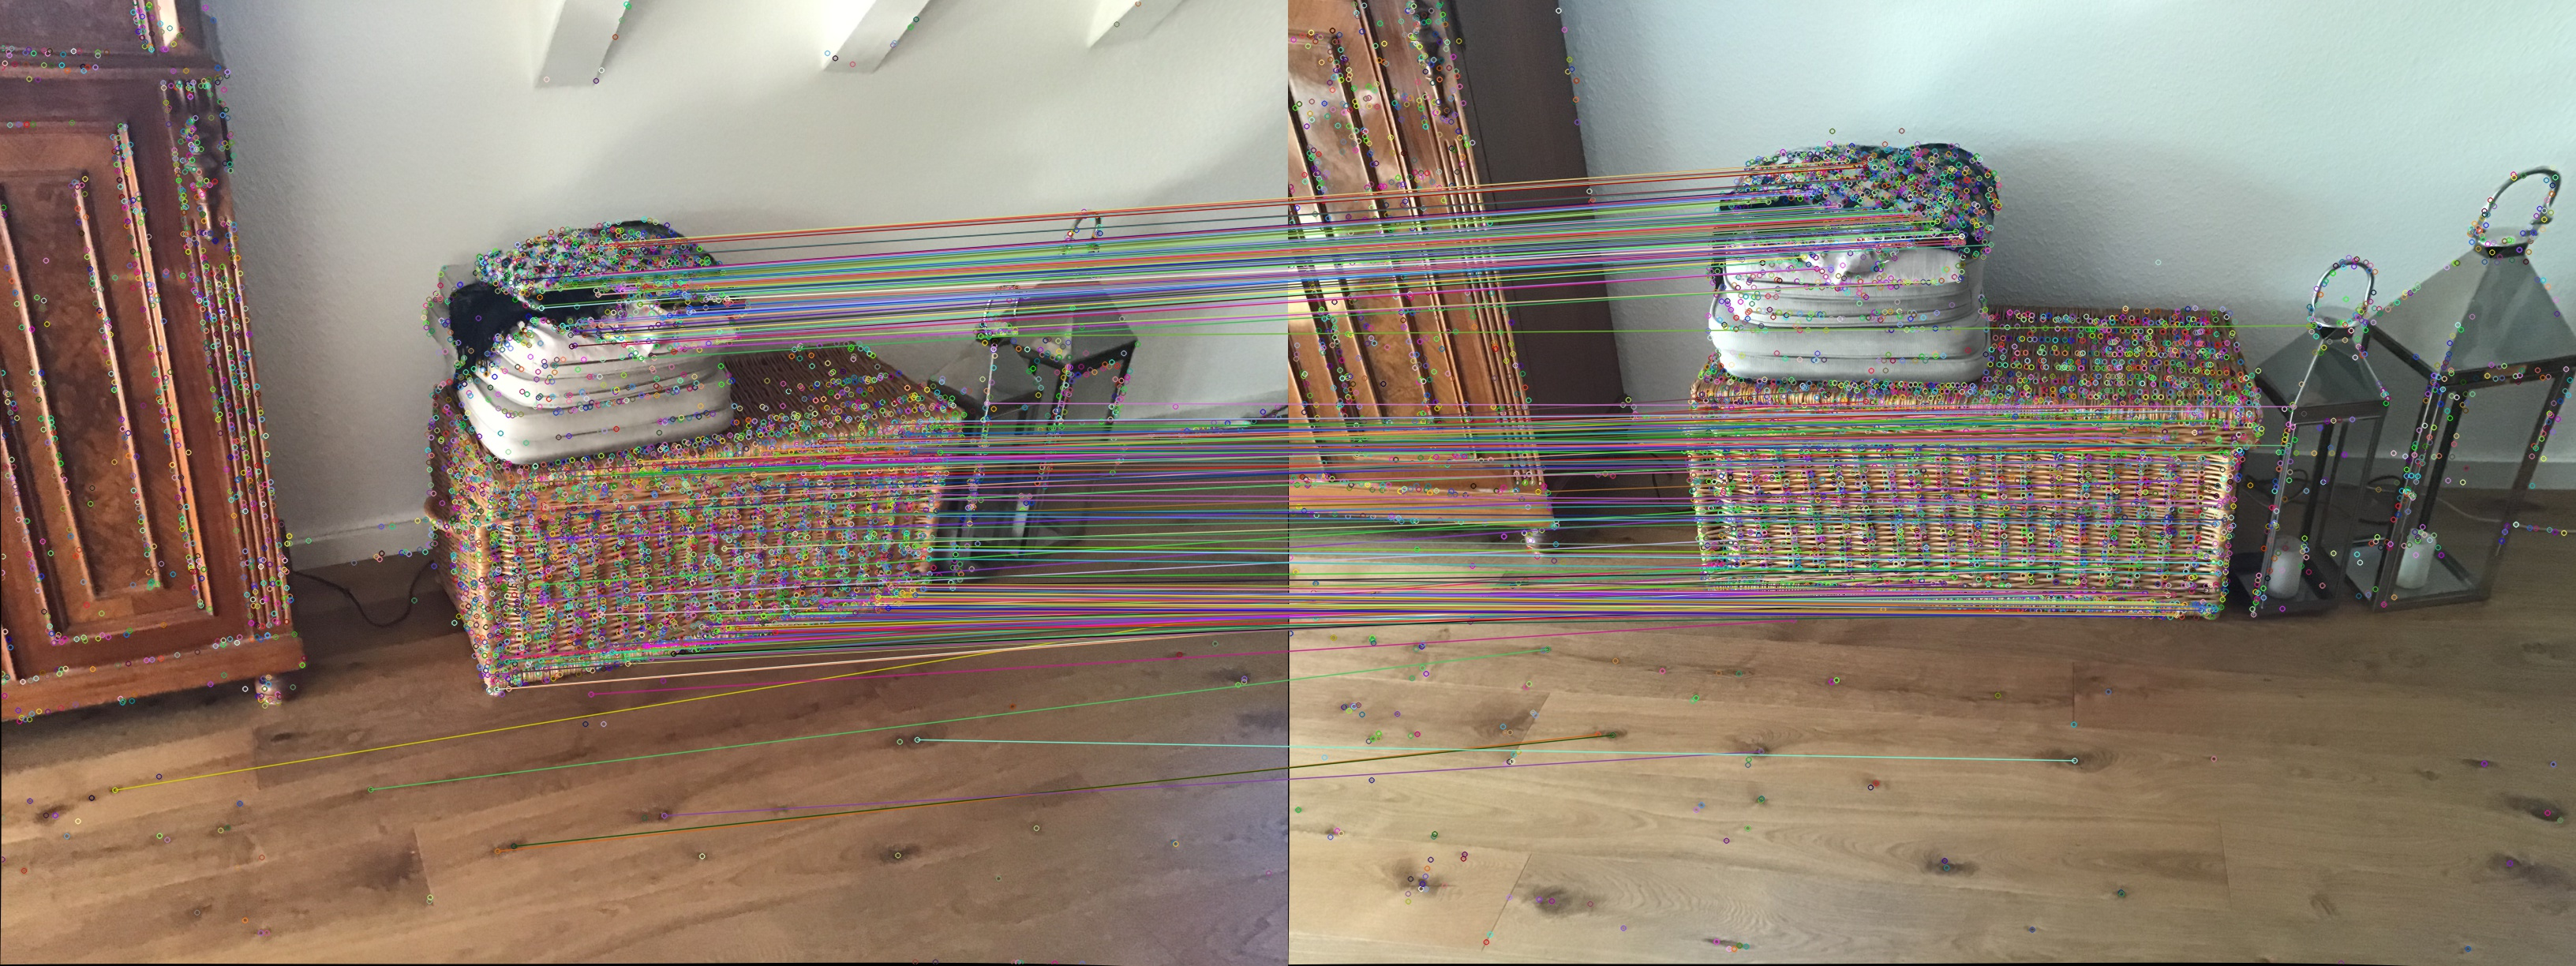
\includegraphics[width=\textwidth]{src/img/box_first_pair_with_matches.jpg}
    \caption{Das erste Bildpaar, mit Matches und Keypoints}
    \label{fig:box-first-pair-with-matches}
\end{figure}

\begin{figure}
    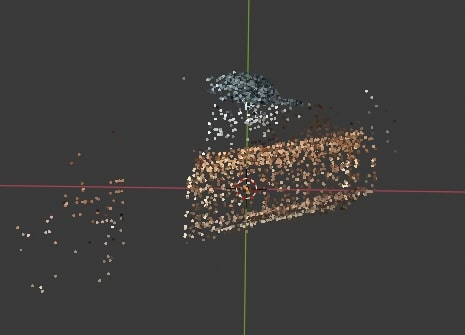
\includegraphics[width=\textwidth]{src/img/box_model.jpg}
    \caption{Die rekonstruierten Punkte aus den Bildern der Box. Das Bild zeigt das Modell ungefähr aus der Position der ersten Kamera.}
    \label{fig:box-model}
\end{figure}

\begin{figure}
    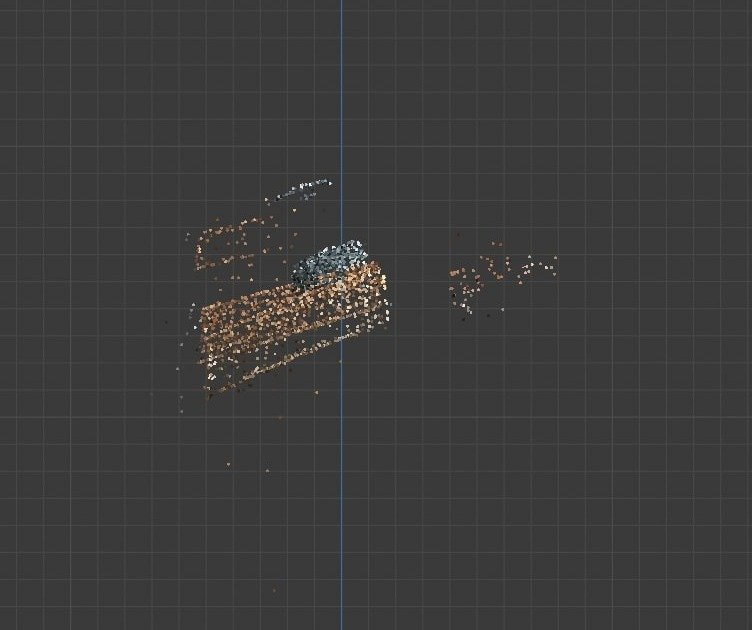
\includegraphics[width=\textwidth]{src/img/box_model_2.jpg}
    \caption{Die rekonstruierten Punkte aus den Bildern der Box. Das Bild zeigt das Modell von der Seite.}
    \label{fig:box-model-2}
\end{figure}
